\documentclass[a0paper,portrait]{baposter}


\usepackage{minipage-marginpar}
\usepackage{wrapfig}
\usepackage{lmodern}
\usepackage{amsmath}
\usepackage[utf8]{inputenc} %unicode support
\usepackage[T1]{fontenc}
\usepackage{tcolorbox}
\usepackage{bm}
\selectcolormodel{cmyk}
\usepackage[font=scriptsize]{caption}
\usepackage{enumitem}

% \graphicspath{{figures/}} % Directory in which figures are stored

\newcommand{\compresslist}{%
\setlength{\itemsep}{0pt}%
\setlength{\parskip}{1pt}%
\setlength{\parsep}{0pt}%
}

\renewcommand{\baselinestretch}{1}

\newenvironment{boenumerate}
  {\begin{enumerate}\renewcommand\labelenumi{\textbf\theenumi.}}
  {\end{enumerate}}

\usepackage{tikz}
\newcommand*\circled[1]{\tikz[baseline=(char.base)]{
            \node[shape=circle,draw,inner sep=2pt] (char) {#1};}}

\begin{document}


\definecolor{darkblue}{cmyk}{0.78,0.78,0,0.56}
\definecolor{lightblue}{cmyk}{0.71,0.46,0,0.41}
\definecolor{silver}{cmyk}{0.08,0.07,0,0.02}

\newtcolorbox{outline}{colback=silver,colframe=darkblue,arc=10pt,
						enlarge top by=1px, enlarge bottom by=1px,
						grow to left by=-10px, grow to right by=-10px}

\newenvironment{myindentpar}[1]%
  {\begin{list}{}%
          {\setlength{\leftmargin}{#1}}%
          \item[]%
  }
  {\end{list}}



\begin{poster}
{
grid=false,
headerborder=open, % Adds a border around the header of content boxes
colspacing=1em, % Column spacing
bgColorOne=white, % Background color for the gradient on the left side of the poster
bgColorTwo=white, % Background color for the gradient on the right side of the poster
borderColor=darkblue, % Border color
headerColorOne=lightblue, % Background color for the header in the content boxes (left side)
headerColorTwo=lightblue, % Background color for the header in the content boxes (right side)
headerFontColor=white, % Text color for the header text in the content boxes
boxColorOne=white, % Background color of the content boxes
textborder=rounded, %rectangle, % Format of the border around content boxes, can be: none, bars, coils, triangles, rectangle, rounded, roundedsmall, roundedright or faded
eyecatcher=false, % Set to false for ignoring the left logo in the title and move the title left
headerheight=0.11\textheight, % Height of the header
headershape=rounded, % Specify the rounded corner in the content box headers, can be: rectangle, small-rounded, roundedright, roundedleft or rounded
headershade=plain,
headerfont=\Large\textsf, % Large, bold and sans serif font in the headers of content boxes
%textfont={\setlength{\parindent}{1.5em}}, % Uncomment for paragraph indentation
linewidth=2pt % Width of the border lines around content boxes
}
{}
%
%----------------------------------------------------------------------------------------
%	TITLE AND AUTHOR NAME
%----------------------------------------------------------------------------------------
%
%
{
\textsf %Sans Serif
{
\vspace{1em}\\
Bayesian Trees and Causality. \\
\vspace{0.1mm}\\
\LARGE -- A semiparametric modeling approach using Bayesian additive regression trees with an application to evaluate heterogeneous treatment effects.\\
}
}
{\indent \sf \footnotesize $\text{Bret Zeldow}^1, \text{Vincent Lo Re III}^2, \text{Jason Roy}^3$
\\
\text{\scriptsize
1. Department of Health Care Policy, Harvard Medical School, 
2. Department of Medicine, University of Pennsylvania, 
3. Department of Biostatistics and Epidemiology, Rutgers School of Public Health}
\vspace{0.5em}\\

%\vspace{0.2em}\\
%
}
{\vspace{3em}\\

\includegraphics[scale=0.9]{logo.jpg}} % University/lab logo


\renewcommand{\baselinestretch}{1.1}

\headerbox{1. Introduction and Causality}{name=introduction,column=0,row=0, span=3}{

\begin{wrapfigure}{r}{0.25\textwidth}
    \vspace{-10pt}
    \begin{center}
        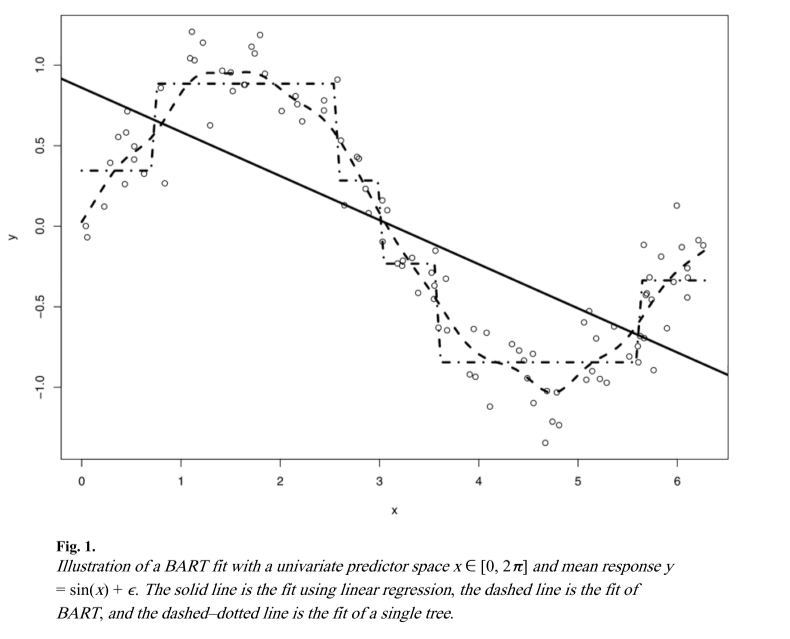
\includegraphics[width=0.8\linewidth]{./images/figure1.png}
    \end{center}
    %\vspace{-145pt}
\end{wrapfigure}

\textbf{a) Overview:} 

- Challenges in prescription of the correct drug for people with HIV persist, specifically for those with co-morbidities.

- In the US 25\% of those with HIV also have Hepatitis-C (HCV) which can lead to liver failure

- Improving HIV-related symptoms has a negative overall effect when it is accompanied by a fatal decline in liver function.

- In previous work, it was discovered that increased cumulative exposure to mtNRTIs (mitochondrial toxic nucleoside reverse transcriptase inhubator) imposes higher risk of decompensation and death \cite{}.

- In this article, the results are extended to a potential modifier of the effect FIB-4 (fibrinogen-4).
\\
\textbf{b) The question: Does the effect of mtNRTIs on the risk of death (within two years) change for individuals with varying FIB-4 levels?}
\\
\textbf{c) Model basic idea:} A new model is proposed to solve the above question that is highly interpretable, due to its parametric nature, while also
maintaining the flexibility of nonlinearity on the remaining confounders.
The model is called \textit{semi-BART} and its potential can be seen in Fig 1, where it manages to capture the non-linearity of a sinusoid much better than linear regression and a usual tree \cite{zeldow2019semiparametric}.
}

\headerbox{2. Model}{name=model,span=2,column=0,below=introduction}{ % To reduce this block to 1 column width, remove 'span=2'
The modification of BART proposed in the paper, called semi-BART, partitions the covariates space into $L=L_1 \cup L_2$. One for the covariates that are \textbf{directly} influencing the relevant question ($L_2$), and \textbf{all the other covariates} ($L_1$), that can increase the model accuracy. The treatment and effect-modifiers are modeled in \textbf{linear terms} for interpretability, while the second partition with \textbf{BART} for flexibility.

\vspace{0.2cm}
\begin{outline}
\textbf{Mathematical Formulation}  
\\
\textbf{- BART:} uses sum-of-trees to predict a binary or real-valued target, given some predictors. $Y = \omega(x) + \epsilon,$ where $\epsilon \sim N(0, \sigma^2),$ and $\omega()$ is the unknown function, that relates $X$ to $Y$.
\\
Usually, $\omega(x)=\sum_{j=1}^m\omega_j(x; T_j, M_j)$ where each $\omega_j(x)$ is a tree with $T_j$ parameter that represents the tree structure, and $M_j$ the one for nodes.
\\
MCMC is used, in order to estimate the fixed but unknown $\sigma^2$ hyperparameter of the $\epsilon$ term.
\\
\textbf{- semi-BART:} Usually in research problems, only a few covariates are of scientific interest.
\\
So we write $Y_i = \omega(L_1) + h(L_2,\psi) + \epsilon_i$, where $h()$ is a parametric function of its covariates in $\psi$, estimated using linear regression and $\omega()$ is of unspecified form estimated using BART.
\end{outline}
}

\renewcommand{\baselinestretch}{1.1}
\headerbox{3. Simulation}{name=application,column=2,below=introduction,span=1}{
A comparison of semi-BART was performed on simulated data for $n = 500$ and $n = 5000$ , between semi-BART, BART, GAM (Generalized additive
models) and linear / logistic regression. Since the data were generated from a
known distribution, the bias, $95\%$ CI, and empirical standard deviation could be measured. Various other comparisons have been conducted in the paper, but the results were similar across all of them.
\\
\\
\textbf{- Continuous outcome with binary treatment and no effect modification.}

Table 1 shows that for small $n$, there is some bias, but all the algorithms are biased by the same amount and in the same direction.

\begin{center}
\vspace{-0.2cm}
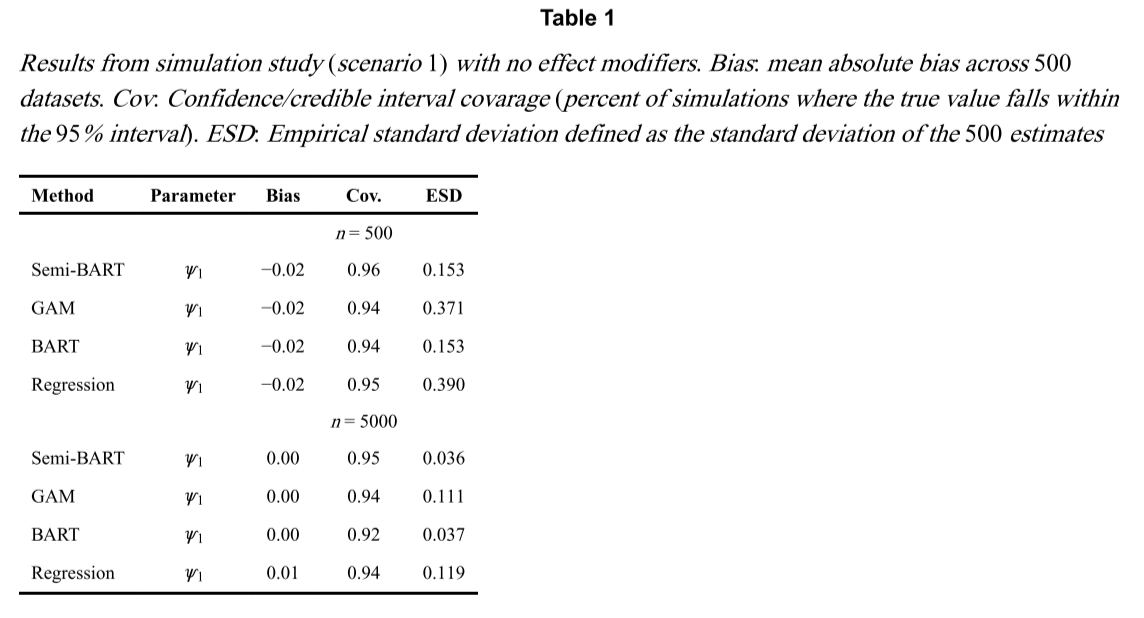
\includegraphics[width=1\linewidth]{./images/table1.png}
\end{center}

\textbf{- Misspecified linear term.}

Table 4 clearly shows that all results are quite similar, but semi-BART has slightly lower ESD.
\begin{flushleft}
\vspace{-0.2cm}
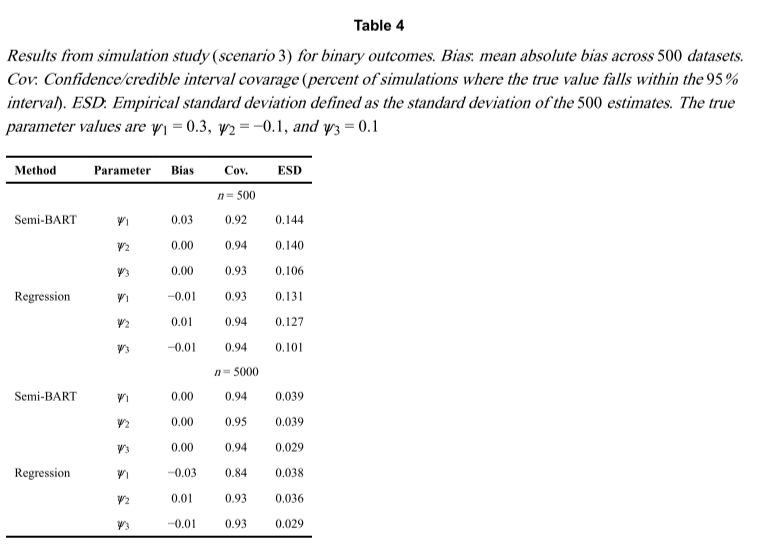
\includegraphics[width=0.95\linewidth]{./images/table4.png}
\end{flushleft}

}



\setlength{\itemsep}{-20pt}%
\renewcommand{\baselinestretch}{1.05}

\headerbox{4. Medical data application}{name=Application,span=2,column=0,below=model,above=bottom}{ % To reduce this block to 1 column width, remove 'span=2'
\vspace{0.2cm}

\begin{wrapfigure}{r}{0.45\textwidth}
    \vspace{-10pt}
    \begin{center}
        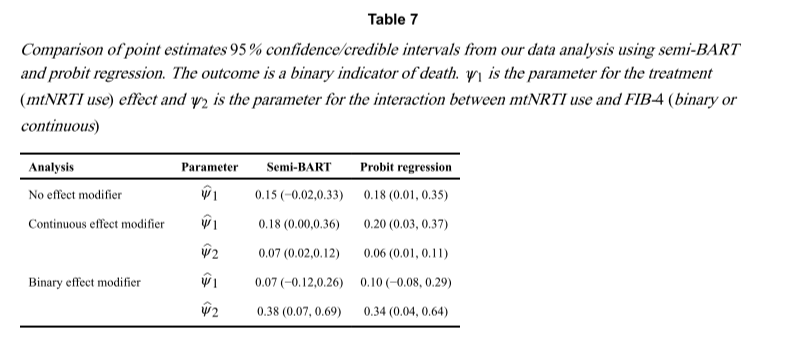
\includegraphics[width=1\linewidth]{./images/table7.png}
    \end{center}
    %\vspace{-145pt}
\end{wrapfigure}

Data are gathered from Veterans Aging Cohort Study (VACS) 2002-2009. The sample consists of patients with HIV/Hepatitis C coinfections. The data contain variables, such as demographics, time of initiation of treatment, HIV characteristics, other laboratory measures etc. The \textbf{outcome} of this analysis is a binary variable, that indicated survival of the patient within the two-year period.
\vspace{1pt}
\begin{itemize}
\item The analysis consisted of $m=50$ trees with $20,000$ iterations.
\item $L$ is partitioned into $L_2$, variables of mtNRTI and the FIB-4 index  and $L_1$, all the other variables.
\end{itemize}
\vspace{2pt}
The three models are
\begin{enumerate}
\item Without continuous effect modifier.
\item With continuous effect modifier.
\item With binary effect modifier.
\end{enumerate}
\vspace{-3pt}
The effect modifier is the FIB-4 index and, the result is:
\\
\textbf{When FIB-4 is present, the effect of mtNRTI is magnified.}

}



\renewcommand{\baselinestretch}{1.0}

\headerbox{5. References}{name=references,column=2,span=1,below=application,above=bottom}{
\tiny % Reduce the font size in this block
\renewcommand{\section}[2]{\vskip 0.01em} % Get rid of the default "References" section title
\bibliographystyle{plain}
\bibliography{assignment_3_bib.bib}
}

\end{poster}

\end{document}